

A raster data structure is a matrix of cells organized into rows
and columns where each cell contains a value representing
information, such as temperature, altitude, population density,
landuse, etc.  This section describes how to display a raster with
two different examples: CM-SAF irradiation rasters will illustrate
the use of diverging palettes; land cover and population data from
the NEO-NASA project will exemplify the display of categorical
data and multivariate rasters.

\section{Diverging palettes}
\label{sec-1}



The \texttt{RasterLayer} object of annual averages of irradiation
estimated by CM-SAF can be easily displayed with the \texttt{levelplot}
method of the \texttt{rasterVis} package.

\index{Packages!raster@\texttt{raster}}
\index{Packages!rasterVis@\texttt{rasterVis}}
\index{levelplot@\texttt{levelplot}}
\index{rasterTheme@\texttt{rasterTheme}}

\lstset{language=R}
\begin{lstlisting}
library(raster)
library(rasterVis)
SISav <- raster('data/SISav')
levelplot(SISav)
\end{lstlisting}

\begin{figure}[h!]
\centering
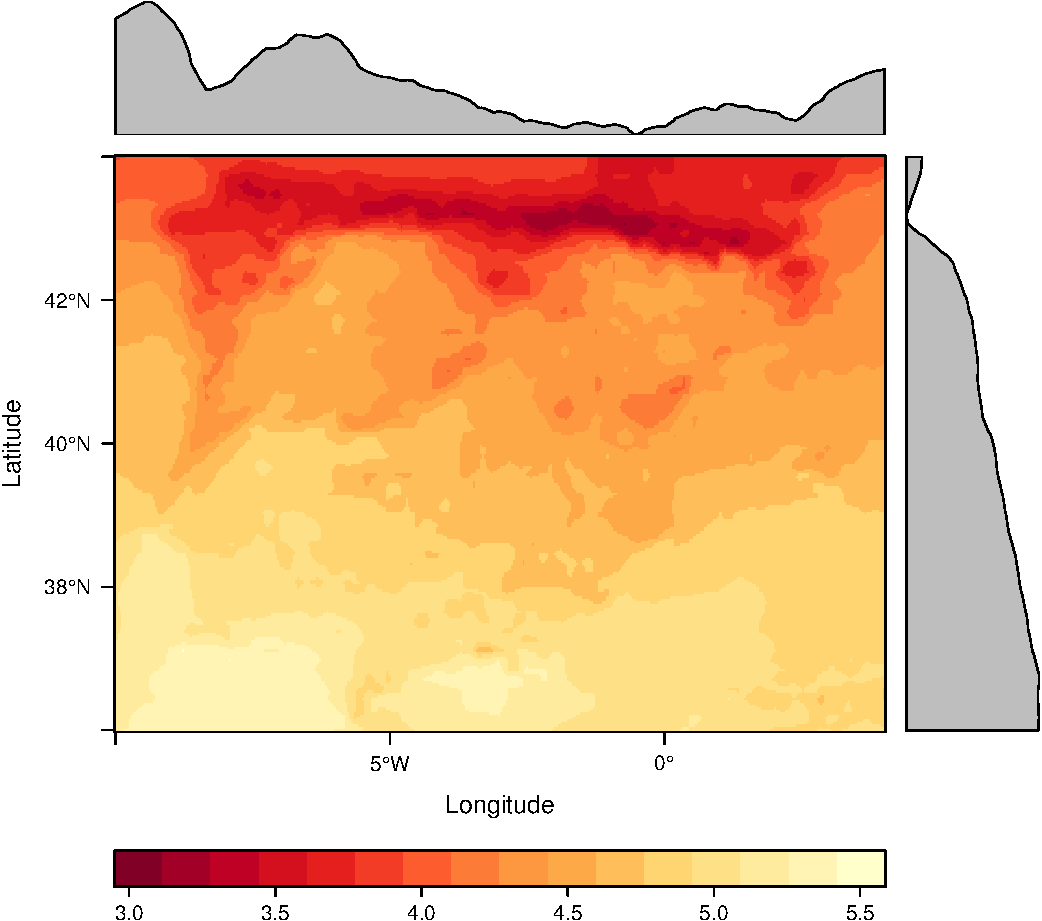
\includegraphics[width=0.8\textwidth]{figs/leveplotSISavOrig.pdf}
\caption{\label{fig:levelplotCMSAF}Annual average of solar radiation displayed with a sequential palette.}
\end{figure}

However, instead of displaying the absolute values of each cell we
will analyze the differences between each cell and the global
average value. This average is computed with the \texttt{cellStats}
function and substracted from the original \texttt{RasterLayer}. The
figure \ref{fig:xyplotSISav} displays the relation between these
scaled values and latitude (\texttt{y}), with 5 different groups defined
by the longitude (\texttt{cut(x, 5)}). It is evident that larger
irradiation values are associated with lower latitudes. However,
there is not such a clear relation between irradiation and
longitude.

\index{cellStats@\texttt{cellStats}}

\lstset{language=R}
\begin{lstlisting}
meanRad <- cellStats(SISav, 'mean')
SISav <- SISav - meanRad
\end{lstlisting}

\index{xyplot@\texttt{xyplot}}
\index{rasterTheme@\texttt{rasterTheme}}
\index{Packages!hexbin@\texttt{hexbin}}
\index{plinrain@\texttt{plinrain}}

\lstset{language=R}
\begin{lstlisting}
xyplot(layer ~ y, data = SISav,
       groups=cut(x, 5),
       par.settings=rasterTheme(symbol=plinrain(n=5, end=200)),
       xlab = 'Latitude', ylab = 'Solar radiation (scaled)',  
       auto.key=list(space='right', title='Longitude', cex.title=1.3))
\end{lstlisting}

\begin{figure}[h!]
\centering
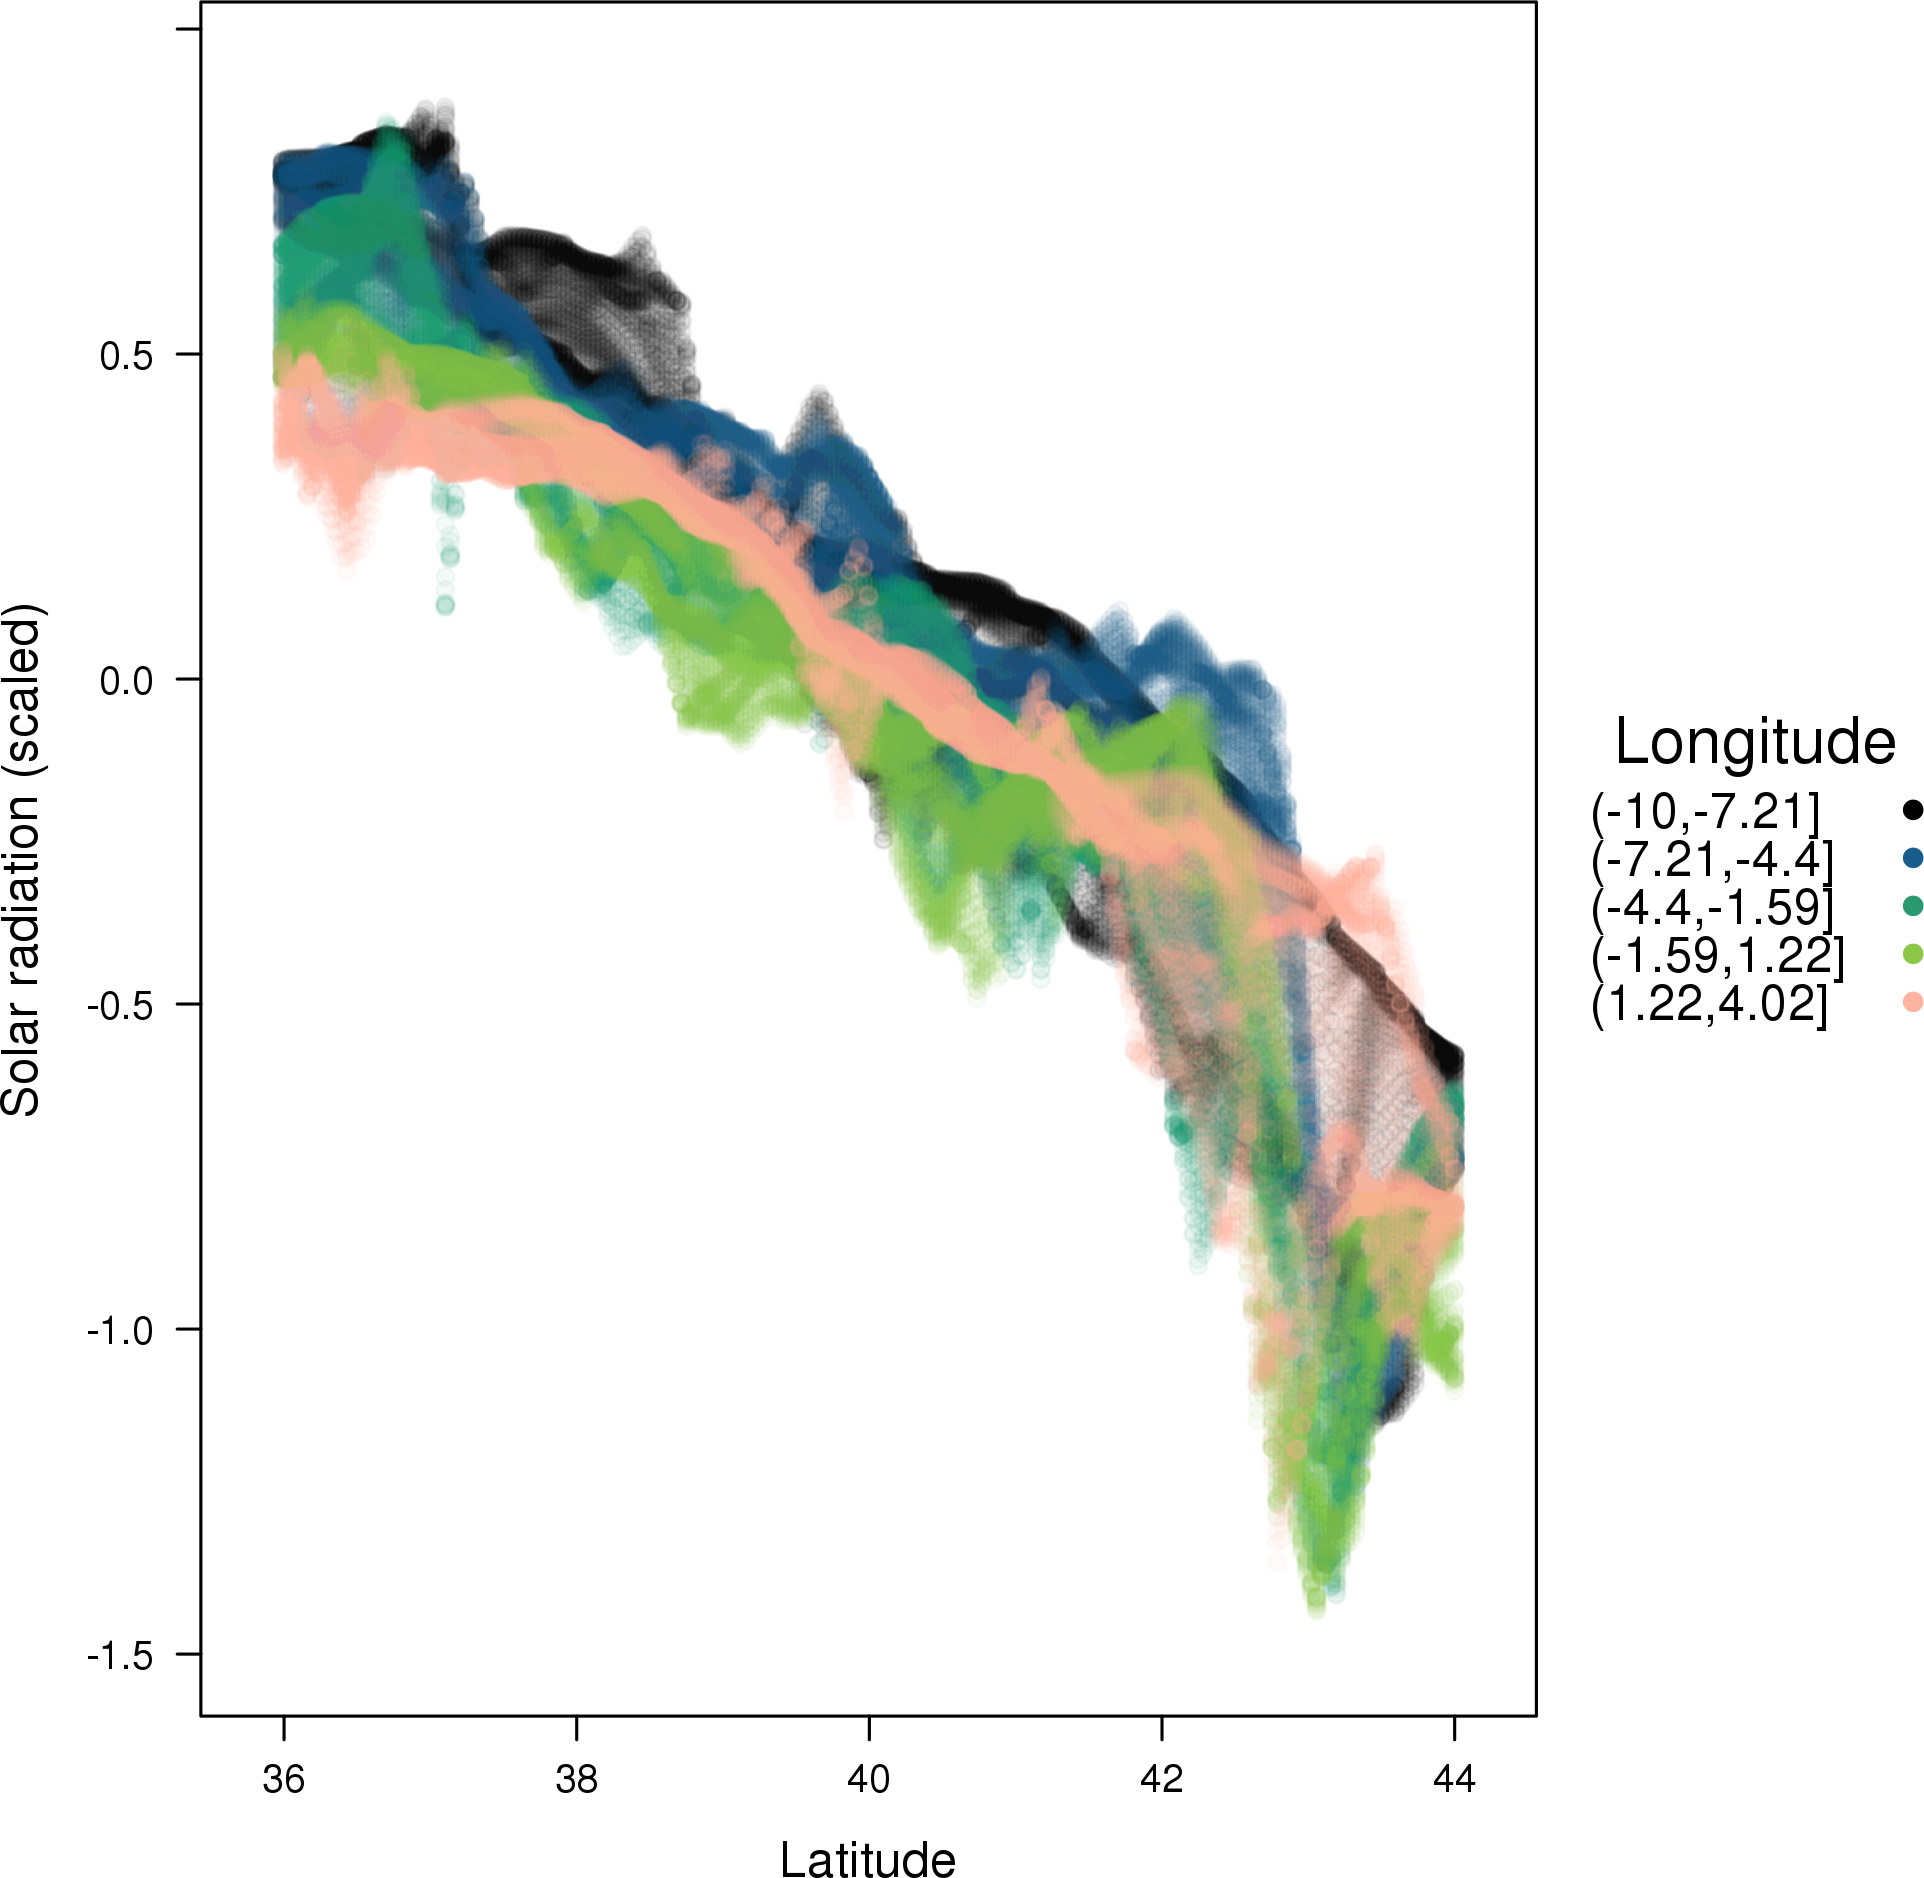
\includegraphics[width=0.8\textwidth]{figs/xyplotSISav.png}
\caption{\label{fig:xyplotSISav}Relation between scaled annual average radiation and latitude for several longitude groups.}
\end{figure}

Numerical information ranging in an interval including a neutral
value is commonly displayed with diverging palettes. These
palettes represent neutral classes with light colors, while low
and high extremes of the data range are highlighted using dark
colors with contrasting hues. I use the Purple-Orange palette from
ColorBrewer with purple for positive values and orange for
negative values. In order to underline the position of the
interval containing zero, the center colour of this palette is
substituted with pure white. The resulting palette is displayed in
the figure \ref{fig:showDivPal} with the custom \texttt{showPal}
function. The correspondent raster map produced with this palette
is displayed in the figure \ref{fig:divPal_SISav_naive}.  Although
extreme positive and negative values can be easily discriminated,
the zero value is not associated with white because the data range
is not symmetrical around zero.

\index{Package!RColorBrewer@\texttt{RColorBrewer}}
\index{brewer.pal@\texttt{brewer.pal}}

\lstset{language=R}
\begin{lstlisting}
divPal <- brewer.pal(n=9, 'PuOr')
divPal[5] <- "#FFFFFF"

showPal <- function(pal, labs=pal, cex=0.6, ...){
  barplot(rep(1, length(pal)), col=pal,
          names.arg=labs, cex.names=cex,
          axes=FALSE, ...)
}

showPal(divPal)
\end{lstlisting}

\begin{figure}[h!]
\centering
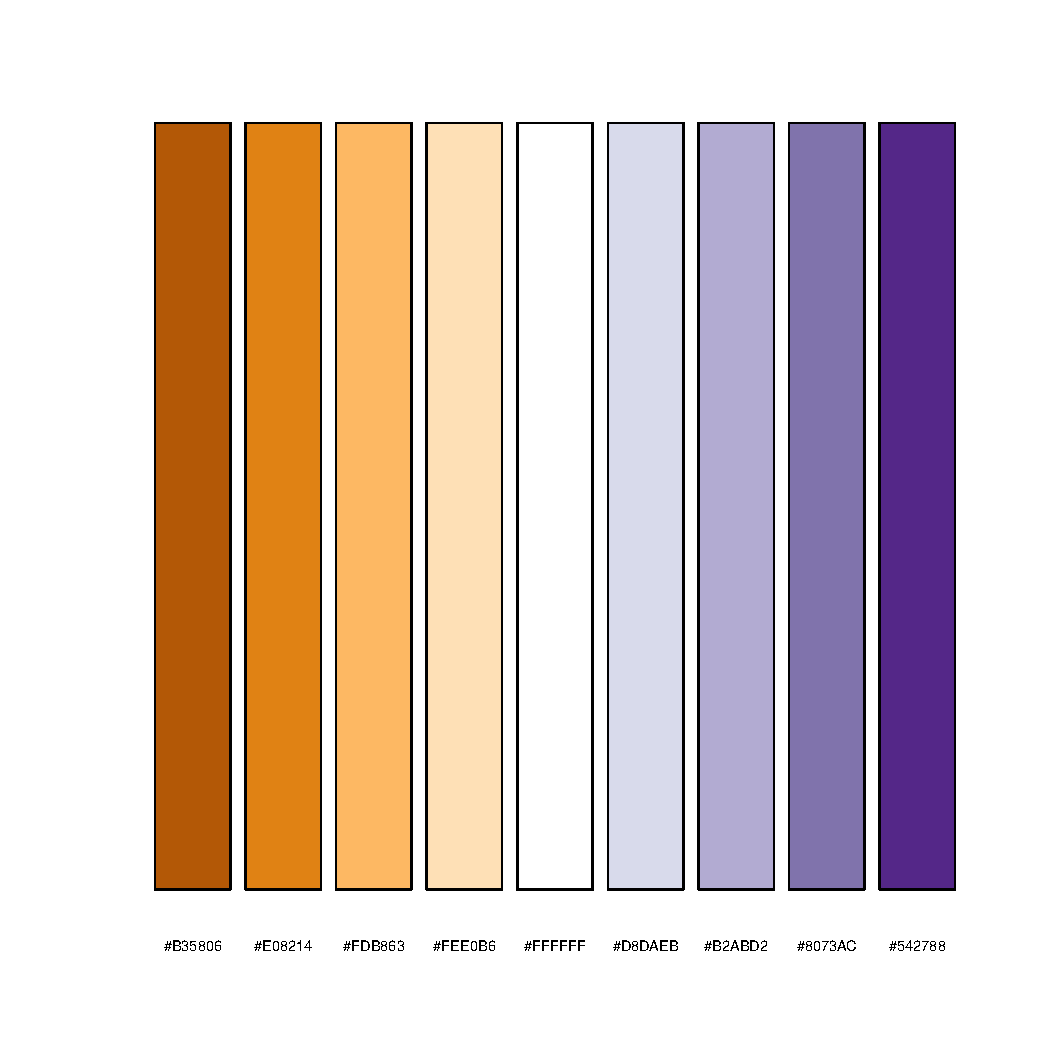
\includegraphics[width=0.35\textwidth]{figs/showDivPal.pdf}
\caption{\label{fig:showDivPal}Purple-Orange diverging palette using white as middle color.}
\end{figure}



\lstset{language=R}
\begin{lstlisting}
divTheme <- rasterTheme(region=divPal)

levelplot(SISav, contour=TRUE, par.settings=divTheme)
\end{lstlisting}

\begin{figure}[h!]
\centering
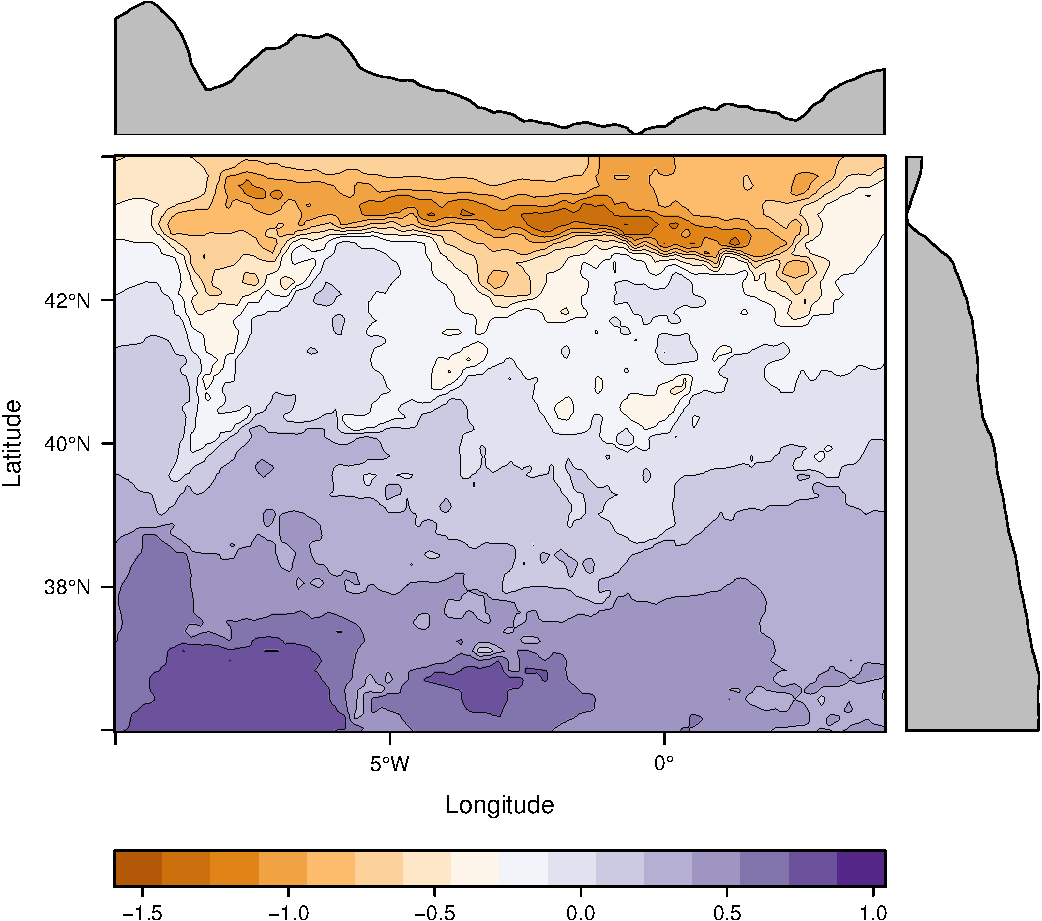
\includegraphics[width=0.8\textwidth]{figs/divPal_SISav_naive.pdf}
\caption{\label{fig:divPal_SISav_naive}Asymmetric raster data (scaled annual average irradiation) displayed with a symmetric diverging palette.}
\end{figure}

The solution is to connect the symmetrical colour palette with the
asymmetrical data range. The first step is to create a set of
breaks such that the zero value is the center of one of the
intervals.

\lstset{language=R}
\begin{lstlisting}
rng <- range(SISav[])
## Number of desired intervals
nInt <- 15
## Increment correspondent to the range and nInt
inc0 <- diff(rng)/nInt
## Number of intervals from the negative extreme to zero
n0 <- floor(abs(rng[1])/inc0)
## Update the increment adding 1/2 to position zero in the center of an interval
inc <- abs(rng[1])/(n0 + 1/2)
## Number of intervals from zero to the positive extreme
n1 <- ceiling((rng[2]/inc - 1/2) + 1)
## Collection of breaks
breaks <- seq(rng[1], by=inc, length= n0 + 1 + n1)
\end{lstlisting}

Next step is to compute the midpoints of each interval. These
points represent the data belonging to each interval and their
value will be connected with a color of the palette.
\index{findInterval@\texttt{findInterval}}
\index{tapply@\texttt{tapply}}

\lstset{language=R}
\begin{lstlisting}
## Midpoints computed with the median of each interval
idx <- findInterval(SISav[], breaks, rightmost.closed=TRUE)
mids <- tapply(SISav[], idx, median)
## Maximum of the absolute value both limits
mx <- max(abs(breaks))
mids
\end{lstlisting}

A simple method to relate the palette and the intervals is with a
straight line such that a point is defined by the absolute maximum
value, (\texttt{(mx, 1)}), and another point by zero, (\texttt{(0, 0.5)}).  Why
are we using the interval [0, 1] as the \texttt{y} coordinate of this
line, and why is 0.5 the result of zero? The reason is that the
input of the \texttt{break2pal} function will be the result of
\texttt{colorRamp}, a function that creates another interpolating
function that maps colors with values between 0 and 1. Therefore,
a new palette is created extracting colors from the original
palette, such that the central color (white) is associated with
the interval containing zero. This palette is displayed in the
figure \ref{fig:showBreak2Pal}.

The raster map produced with this new palette is displayed in the
figure \ref{fig:divPalSISav}. Now zero is clearly associated with the
white color.
\index{colorRamp\texttt{colorRamp}}
\index{rgb@\texttt{rgb}}

\lstset{language=R}
\begin{lstlisting}
break2pal <- function(x, mx, pal){
  ## x = mx gives y = 1
  ## x = 0 gives y = 0.5
  y <- 1/2*(x/mx + 1)
  rgb(pal(y), maxColorValue=255)
}

## Interpolating function that maps colors with [0, 1]
## rgb(divRamp(0.5), maxColorValue=255) gives "#FFFFFF" (white)
divRamp <- colorRamp(divPal)
## Diverging palette where white is associated with the interval
## containing the zero
pal <- break2pal(mids, mx, divRamp)
showPal(pal, round(mids, 1))
\end{lstlisting}

\begin{figure}[h!]
\centering
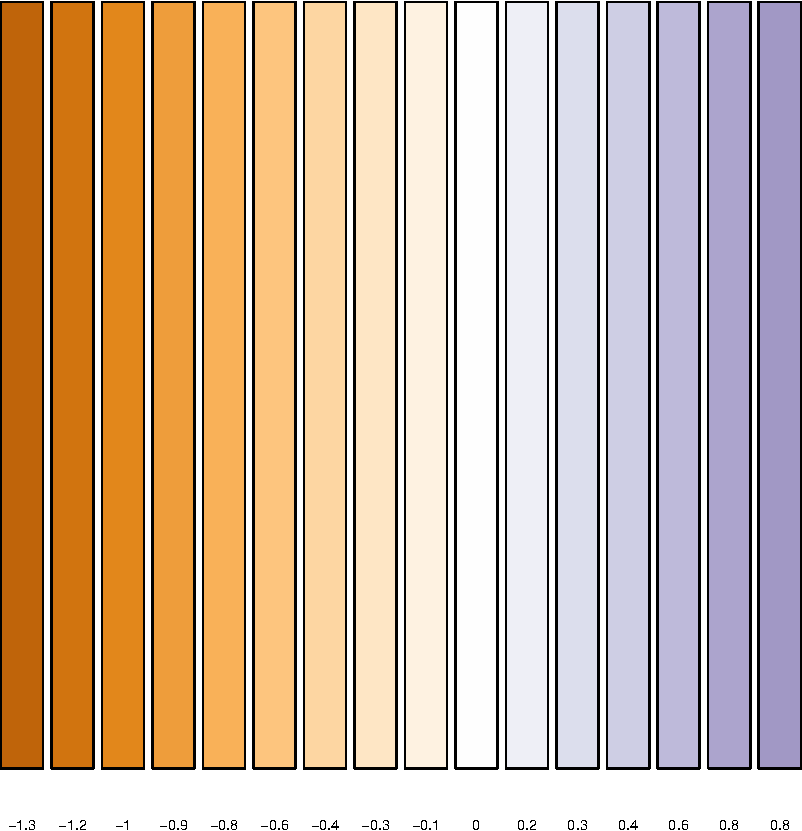
\includegraphics[width=0.5\textwidth]{figs/showBreak2Pal.pdf}
\caption{\label{fig:showBreak2Pal}Modified diverging palette related with the asymmetrical raster data.}
\end{figure}



\lstset{language=R}
\begin{lstlisting}
levelplot(SISav, par.settings=rasterTheme(region=pal),
          at=breaks, contour=TRUE)
\end{lstlisting}

\begin{figure}[h!]
\centering
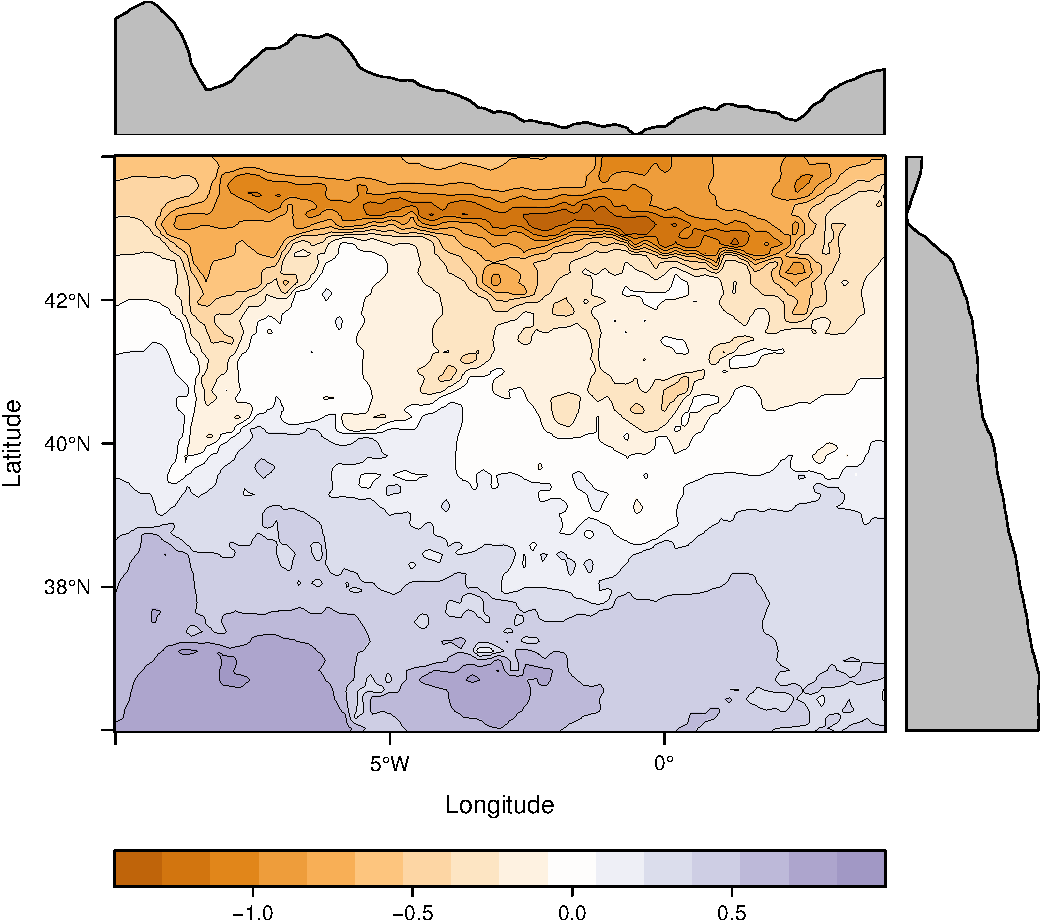
\includegraphics[width=0.8\textwidth]{figs/divPalSISav.pdf}
\caption{\label{fig:divPalSISav}Asymmetric raster data (scaled annual average irradiation) displayed with a modified diverging palette.}
\end{figure}


It is interesting to note two operations carried out internally by
the \texttt{lattice} package. First, the \texttt{custom.theme} function (used by
\texttt{rasterTheme}) creates a new palette with 100 colours using
\texttt{colorRampPalette} to interpolate the palette passed as an
argument. Second, the \texttt{level.colors} function makes the
arrangement between intervals and colors. If this function
receives more colors than intervals, it chooses a subset of the
palette disregarding some of the intermediate colors. Therefore,
since this function will receive 100 colors from \texttt{par.settings} it
is difficult to control exactly which colors of our original
palette will be represented.

An alternative way for finer control is to fill with our palette
the \texttt{regions\$col} component of the theme after it has been
created.


\lstset{language=R}
\begin{lstlisting}
divTheme <- rasterTheme()

divTheme$regions$col <- pal
levelplot(SISav, par.settings=divTheme, at=breaks, contour=TRUE)
\end{lstlisting}

\begin{figure}[h!]
\centering
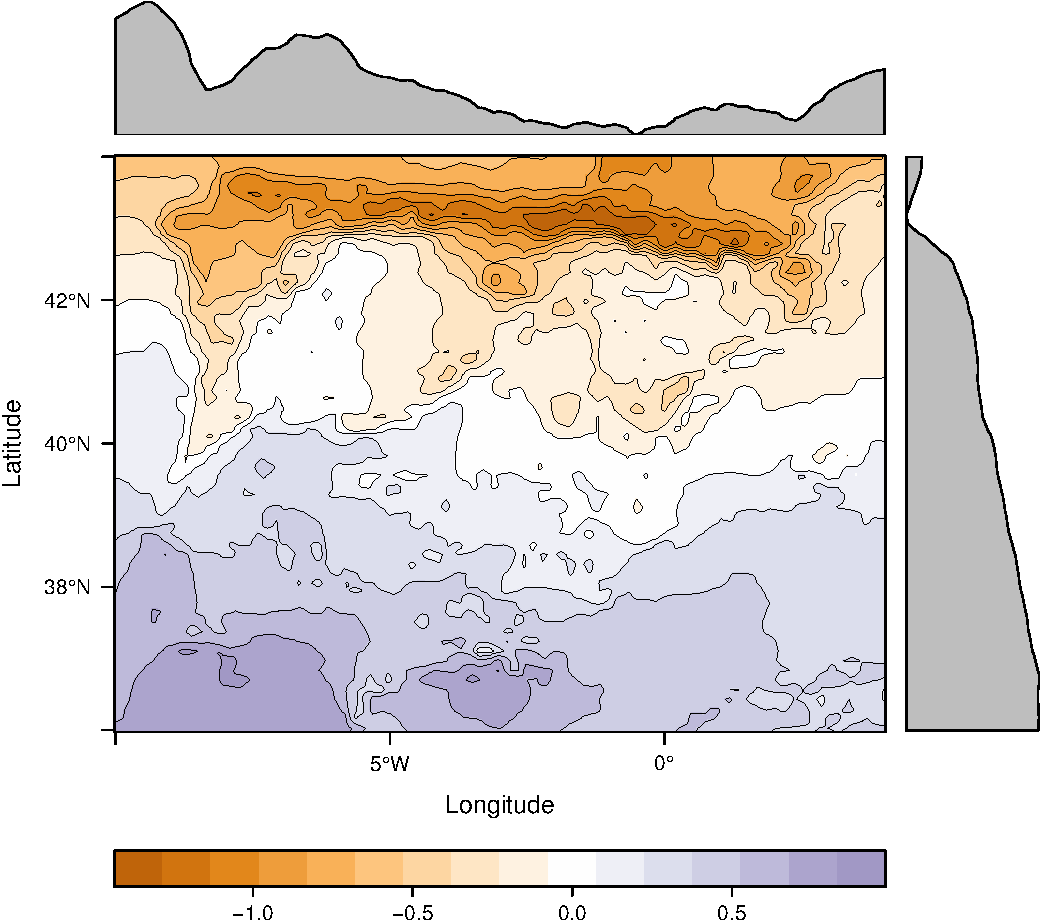
\includegraphics[width=0.8\textwidth]{figs/divPalSISav_regions.pdf}
\caption{\label{fig:divPal_SISav_regions}Same as figure \ref{fig:divPalSISav} but colors are assigned directly to the \texttt{regions\$col} component of the theme.}
\end{figure}

A final improvement to this map is to compute the intervals using
a classification algorithm with the \texttt{classInt} package. With this
approach it is likely that zero will not be perfectly centered in
its correspondent interval. The rest of the code is exactly the
same as above replacing the \texttt{breaks} vector with the result of the
\texttt{classIntervals} function. The figure
\ref{fig:divPalSISav_classInt} displays the result.

\index{Packages!classInt@\texttt{classInt}}
\index{classIntervals@\texttt{classIntervals}}

\lstset{language=R}
\begin{lstlisting}
library(classInt)

cl <- classIntervals(SISav[],
                     ## n=15, style='equal')
                     ## style='hclust')
                     ## style='sd')
                     style='kmeans')
                     ## style='quantile')
cl
breaks <- cl$brks
\end{lstlisting}


\lstset{language=R}
\begin{lstlisting}
idx <- findInterval(SISav[], breaks, rightmost.closed=TRUE)
mids <- tapply(SISav[], idx, median)
mids
mx <- max(abs(breaks))
pal <- break2pal(mids, mx, divRamp)
divTheme$regions$col <- pal
levelplot(SISav, par.settings=divTheme, at=breaks, contour=TRUE)
\end{lstlisting}

\begin{figure}[h!]
\centering
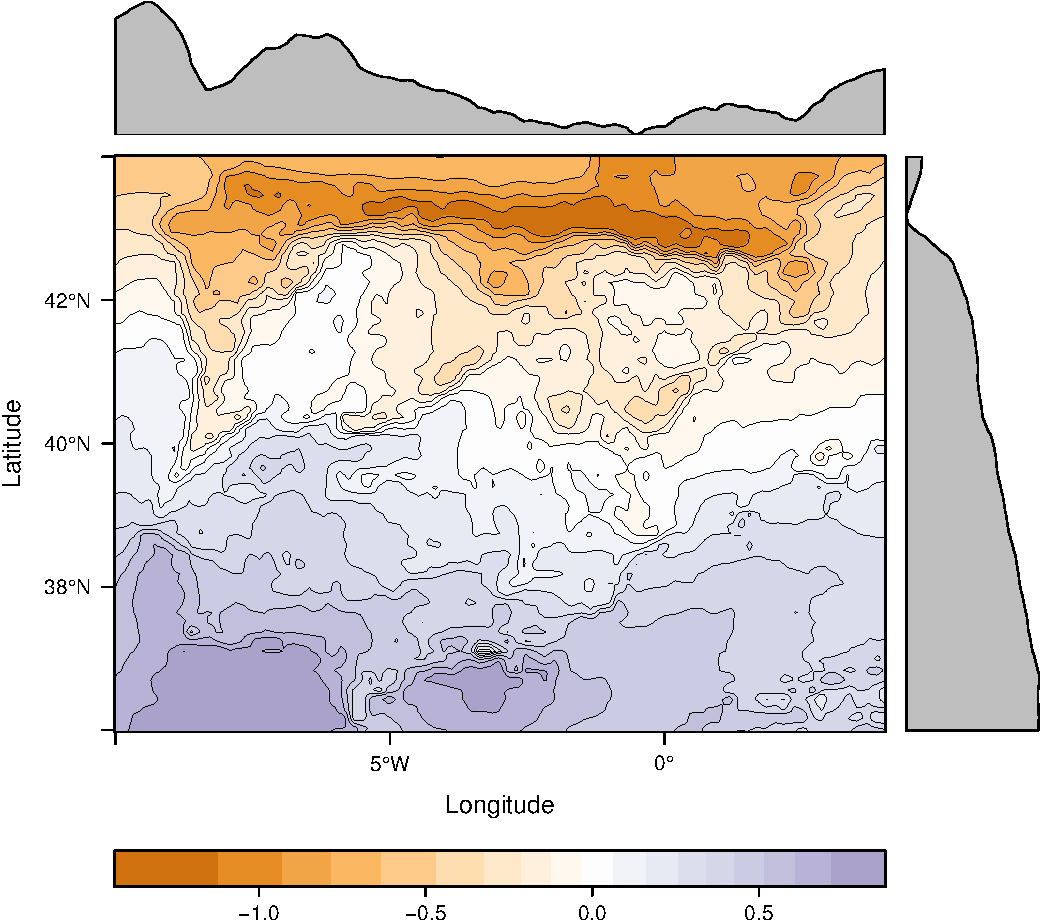
\includegraphics[width=0.8\textwidth]{figs/divPalSISav_classInt.pdf}
\caption{\label{fig:divPalSISav_classInt}Same as figure \ref{fig:divPal_SISav_regions} but defining intervals with the optimal classification method.}
\end{figure}
\section{Categorical data}
\label{sec-2}



Land cover is the observed physical cover on the earth's
surface. A set of 17 different categories is commonly used. Using
satellite observations, it is possible to map where on Earth each of
these 17 land surface categories can be found and how these land
covers change over time. This raster is a typical example of
categorical data. 

This section illustrates how to read and display rasters with
categorical information using information from the NEO-NASA
project. After the land cover and population density files have
been downloaded, two \texttt{RasterLayers} can be created with the
\texttt{raster} package. Both files are read, their geographical extent
reduced to the area of India and China, and cleaned (99999 cells
are replaced with \texttt{NA}).

\index{Packages!raster@\texttt{raster}}
\index{extent@\texttt{extent}}
\index{crop@\texttt{crop}}

\lstset{language=R}
\begin{lstlisting}
library(raster)
## China and India  
ext <- extent(65, 135, 5, 55)

pop <- raster('875430rgb-167772161.0.FLOAT.TIFF')
pop <- crop(pop, ext)
pop[pop==99999] <- NA

landClass <- raster('241243rgb-167772161.0.TIFF')
landClass <- crop(landClass, ext)
\end{lstlisting}



The codes of the classification are graphically described in the
figure \ref{fig:lccKey}. In summary, the sea is labeled with 0,
forests with 1 to 5, shrublands, grasslands and wetlands with 6 to
11, agriculture and urban lands with 12 to 14, and snow and barren
with 15 and 16.  These four groups (sea is replaced \texttt{NA}) will be
the levels of the categorical raster. The \texttt{raster} package
includes the \texttt{ratify} method to define a layer as categorical data
filling it with integer values associated to a Raster Attribute
Table (RAT).

\begin{figure}
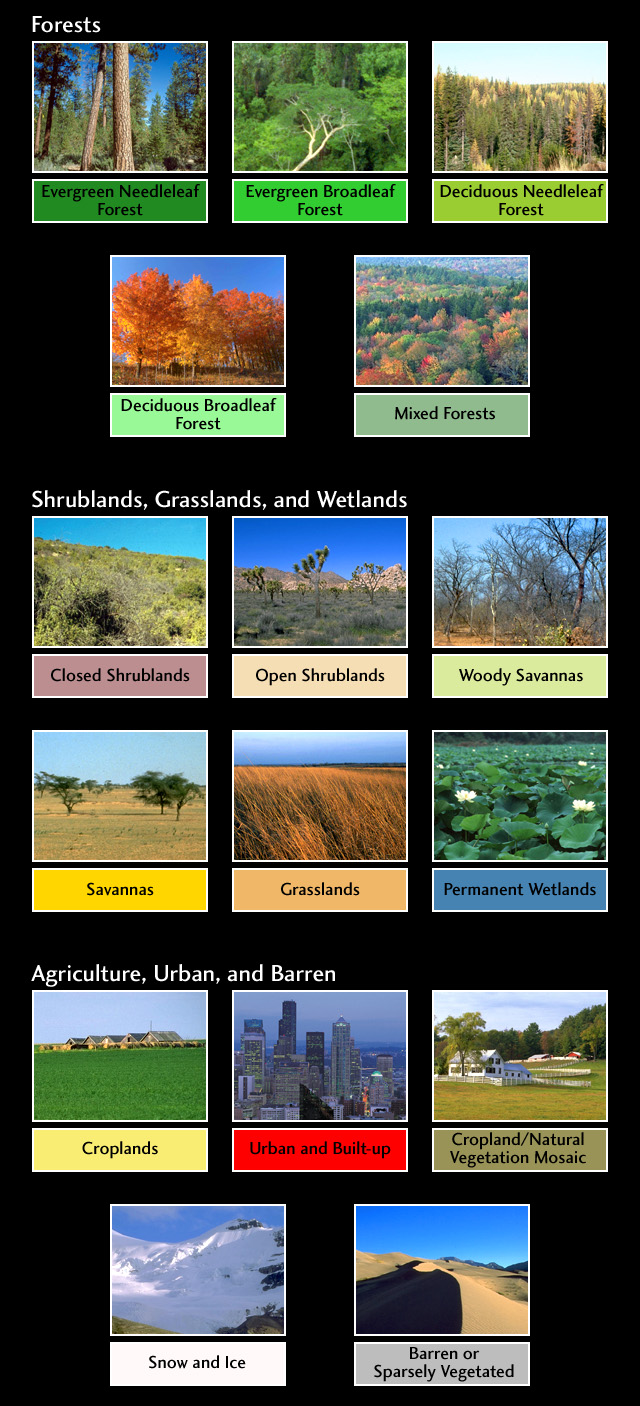
\includegraphics[width=0.3\textwidth]{figs/lcc_key.jpg}
\caption{\label{fig:lccKey}Codes of land cover classification}
\end{figure}

\index{ratify@\texttt{ratify}}
\index{cut@\texttt{cut}}

\lstset{language=R}
\begin{lstlisting}
landClass[landClass %in% c(0, 254)] <- NA
## Only four groups are needed:
## Forests: 1:5
## Shublands, etc: 6:11
## Agricultural/Urban: 12:14
## Snow: 15:16
landClass <- cut(landClass, c(0, 5, 11, 14, 16))
## Add a Raster Atribute Table and define the raster as categorical data
landClass <- ratify(landClass)
## Configure the RAT: first create a RAT data.frame using the
## levels method; second, set the values for each class (to be
## used by levelplot); third, assign this RAT to the raster
## using again levels
rat <- levels(landClass)[[1]]
rat$classes <- c('Forest', 'Land', 'Urban', 'Snow')
levels(landClass) <- rat
\end{lstlisting}

This categorical raster can be easily displayed with the
\texttt{levelplot} method of the \texttt{rasterVis} package. Previously, a theme
is defined with the background color set to \texttt{lightskyblue1} to
display the sea areas (filled with \texttt{NA} values), and the region
palette is defined with adequate colors.

\index{Packages!rasterVis@\texttt{rasterVis}}
\index{levelplot@\texttt{levelplot}}
\index{modifyList@\texttt{modifyList}}
\index{rasterTheme@\texttt{rasterTheme}}

\lstset{language=R}
\begin{lstlisting}
library(rasterVis)

pal <- c('palegreen4', # Forest
         'lightgoldenrod', # Land
         'indianred4', # Urban
         'snow3')      # Snow

catTheme <- modifyList(rasterTheme(),
                       list(panel.background = list(col='lightskyblue1'),
                            regions = list(col= pal)))

levelplot(landClass, maxpixels=3.5e5, par.settings=catTheme,
          panel=panel.levelplot.raster)
\end{lstlisting}

\begin{figure}[h!]
\centering
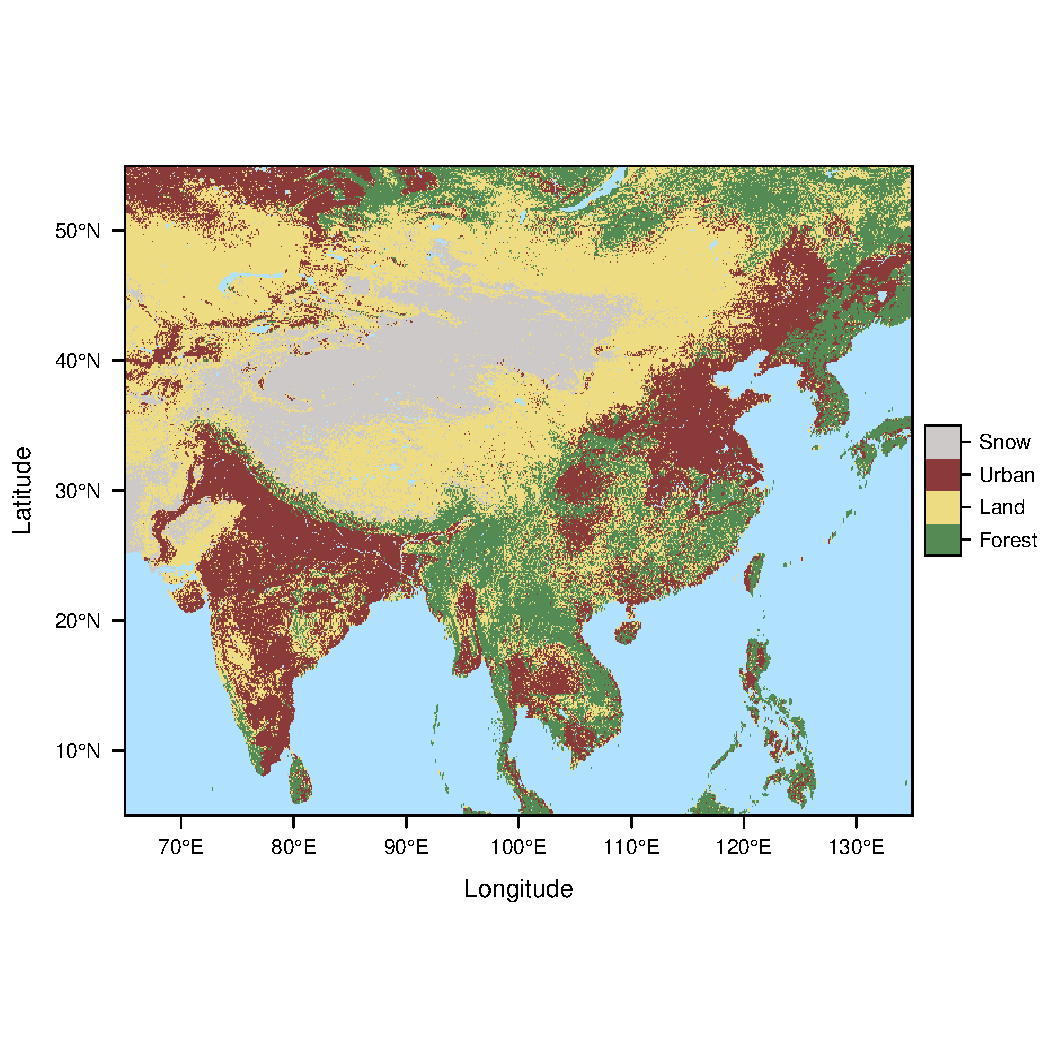
\includegraphics[width=0.8\textwidth]{figs/landClass.pdf}
\caption{\label{fig:landClass}Land cover raster (categorical data).}
\end{figure}

Let's explore the relation between the land cover and population
density rasters. Figure \ref{fig:populationNASA} displays this
last raster using a logarithmic scale.


\lstset{language=R}
\begin{lstlisting}
pPop <- levelplot(pop, zscaleLog=10, par.settings=BTCTheme,
                  maxpixels=3.5e5, panel=panel.levelplot.raster)
pPop
\end{lstlisting}

\begin{figure}[h!]
\centering
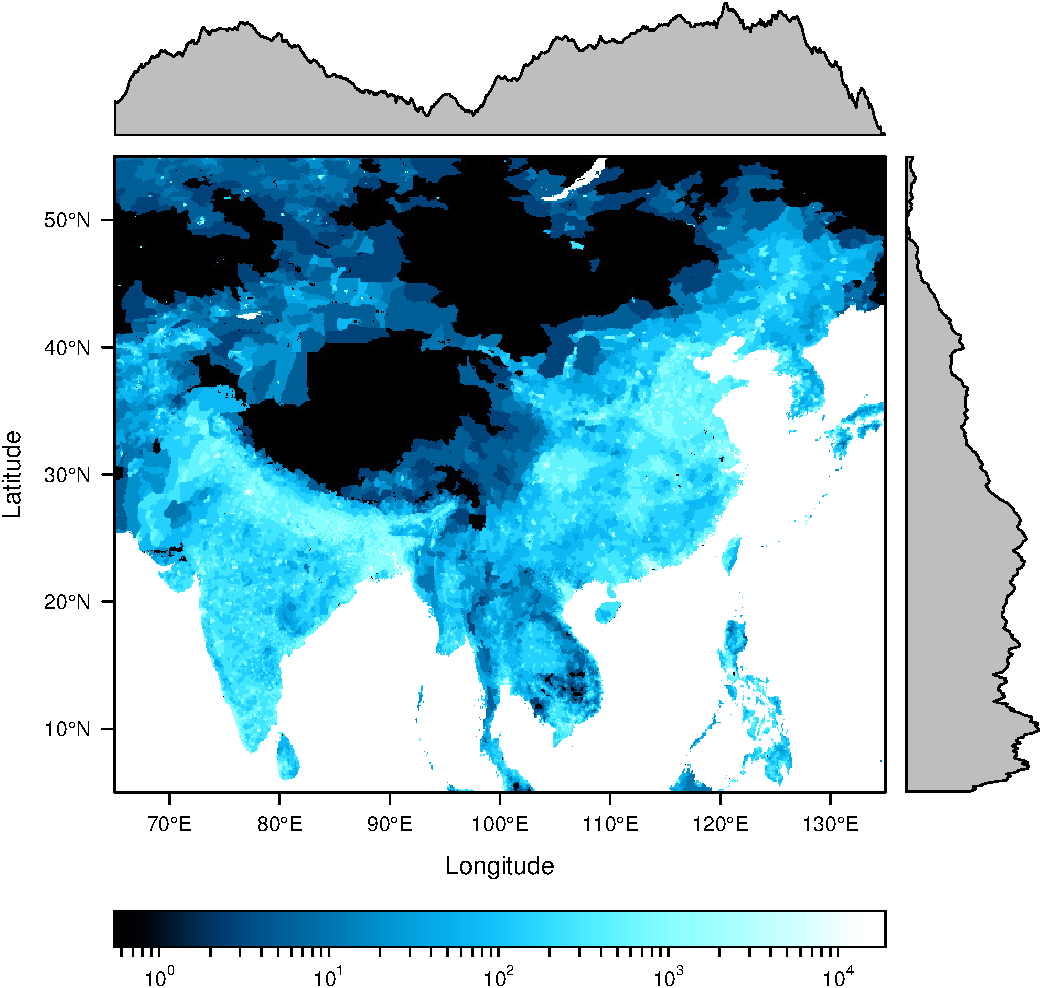
\includegraphics[width=0.8\textwidth]{figs/populationNASA.pdf}
\caption{\label{fig:populationNASA}Population density raster.}
\end{figure}

Both rasters can be joined together with the \texttt{stack} method to
create a new \texttt{RasterStack} object. Figure
\ref{fig:histogramLandClass} displays the distribution of the
logarithm of the population density associated to each land class.

\index{stack@\texttt{stack}}
\index{histogram@\texttt{histogram}}

\lstset{language=R}
\begin{lstlisting}
s <- stack(pop, landClass)
names(s) <- c('pop', 'landClass')
histogram(~log10(pop)|landClass, data=s,
          scales=list(relation='free'))
\end{lstlisting}

\begin{figure}[h!]
\centering
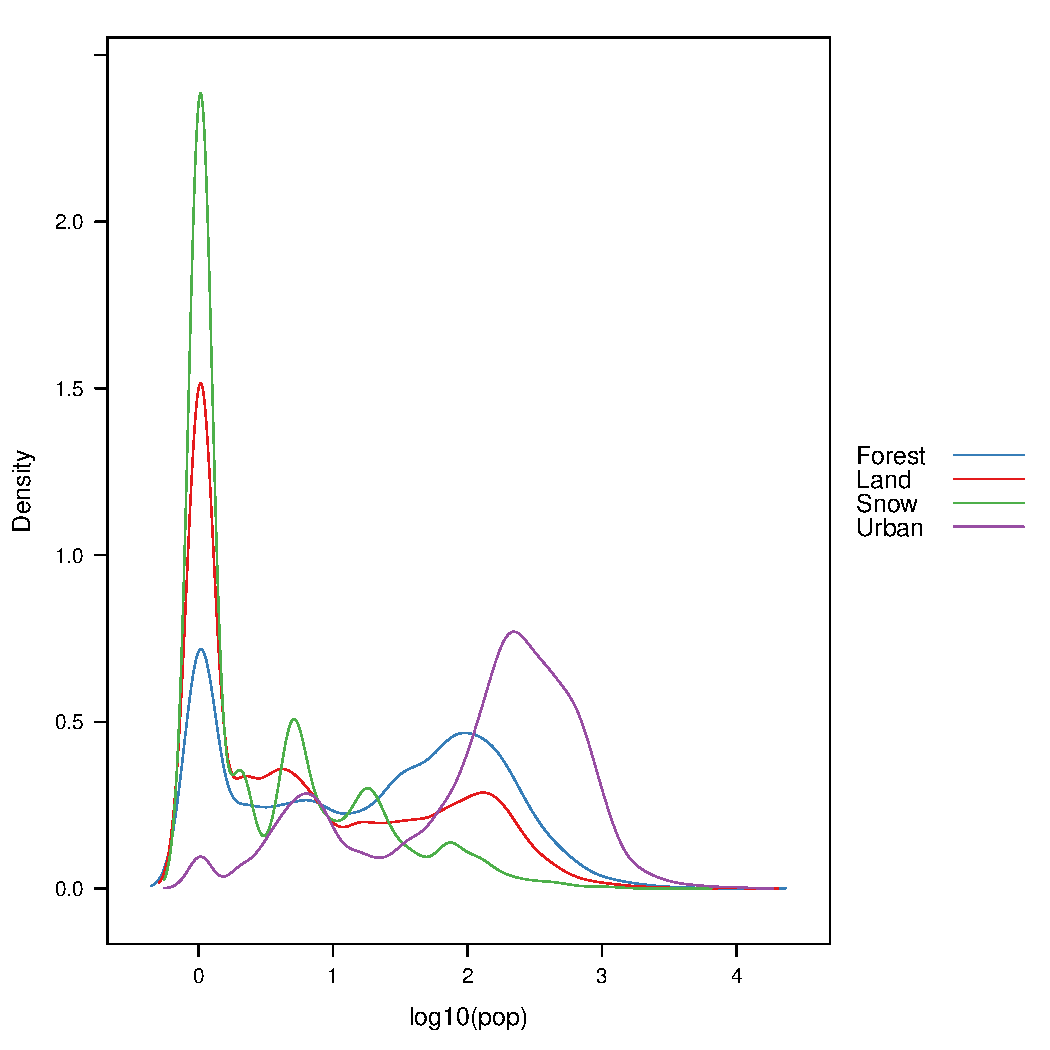
\includegraphics[width=0.8\textwidth]{figs/histogramLandClass.pdf}
\caption{\label{fig:histogramLandClass}Distribution of the logarithm of the population density associated to each land class.}
\end{figure}
\section{\floweroneleft  Multivariate legend}
\label{sec-3}

We can reproduce the code used to create the multivariate
choropleth (section \ref{sec:multiChoropleth}) using the
\texttt{levelplot} function from the \texttt{rasterVis} package. Again, the
result is a list of \texttt{trellis} objects. Each of these objects is
the representation of the population density in a particular land
class. The \texttt{+.trellis} function of the \texttt{latticeExtra} package with
\texttt{Reduce} superposes the elements of this list and produce a
\texttt{trellis} object. Figure \ref{fig:popLandClass} displays the
result.

  



\lstset{language=R}
\begin{lstlisting}
## at for each sub-levelplot is obtained from the global levelplot
at <- pPop$legend$bottom$args$key$at
classes <- rat$classes
nClasses <- length(classes)

pList <- lapply(1:nClasses, function(i){
  landSub <- landClass
  ## Those cells from a different land class are set to NA...
  landSub[!(landClass==i)] <- NA
  ## ... and the resulting raster mask the population raster
  popSub <- mask(pop, landSub)
  ## The HCL color wheel is divided in nClasses
  step <- 360/nClasses
  ## and a sequential palette is constructed with a hue from one
  ## the color wheel parts
  cols <- rev(sequential_hcl(16, h = (30 + step*(i-1))%%360))

  pClass <- levelplot(popSub, zscaleLog=10, at=at, maxpixels=3.5e5,
                      col.regions=cols, margin=FALSE)
})
\end{lstlisting}



\begin{figure}[h!]
\centering
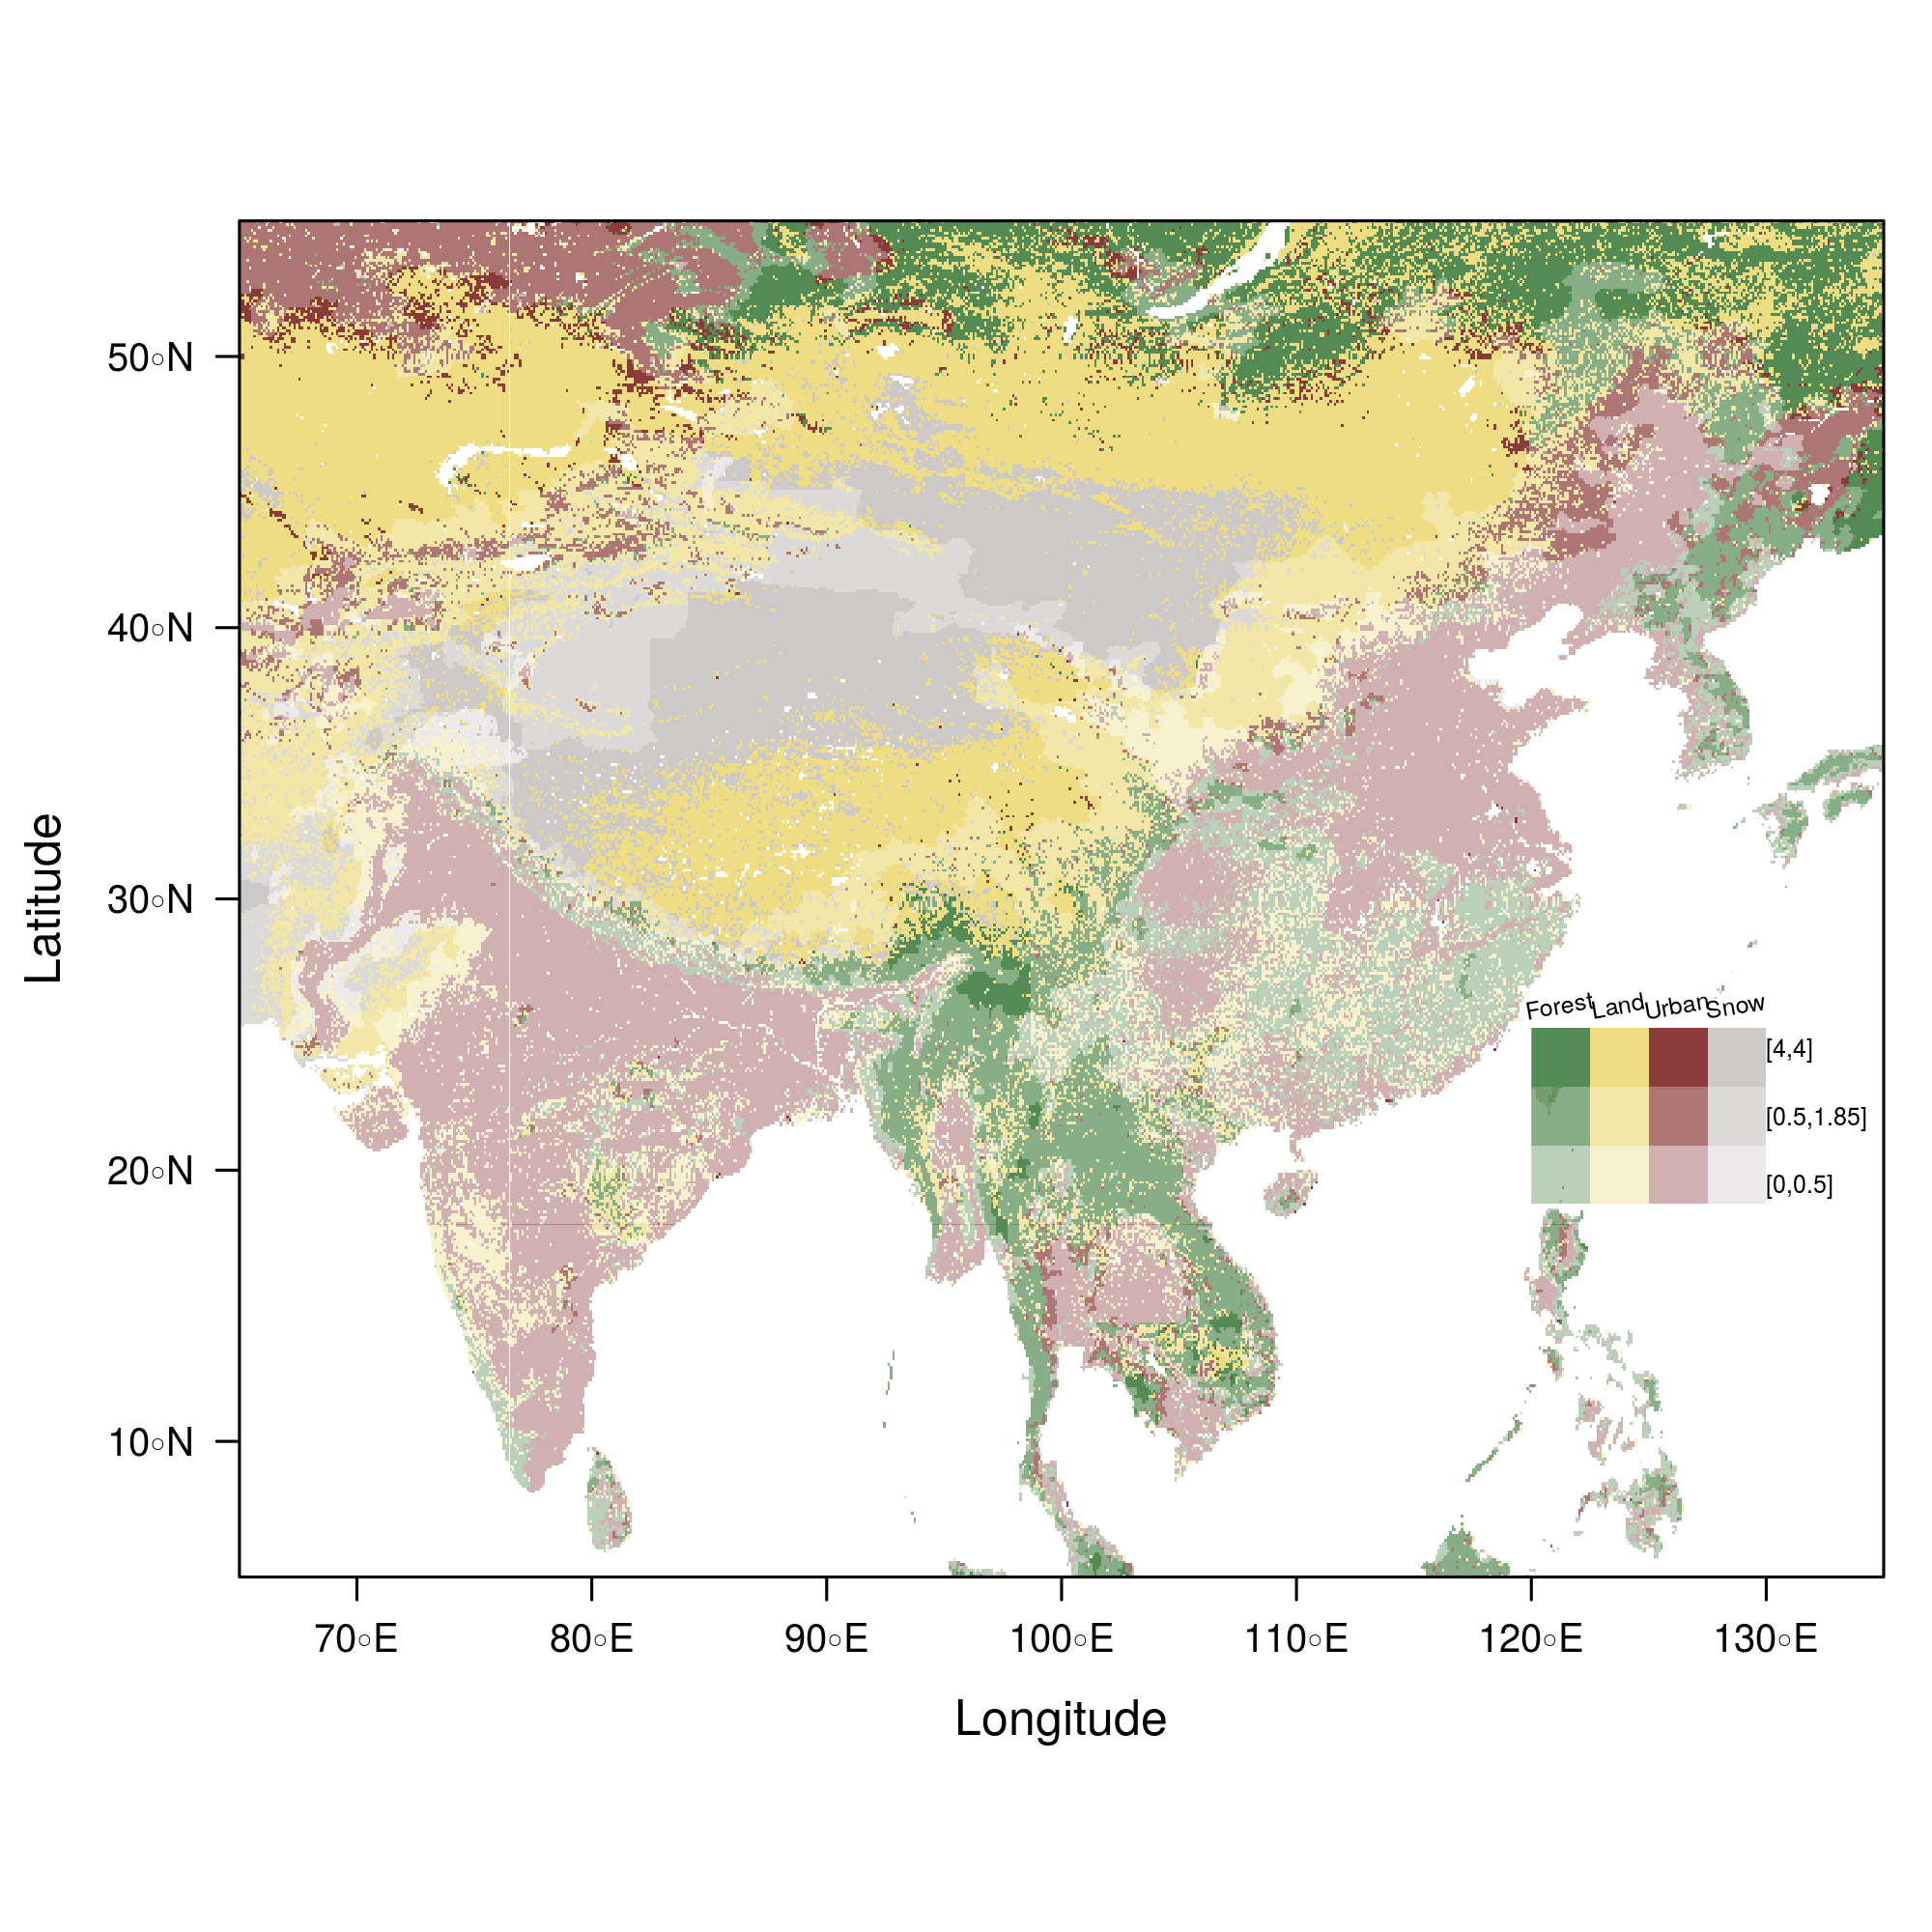
\includegraphics[width=0.8\textwidth]{figs/popLandClass.png}
\caption{\label{fig:popLandClass}Population density for each land class (multivariate raster).}
\end{figure}
